\section{Biology Recap}

% \begin{frame}[c]{The Human Brain in Numbers}
%     \normalsize
%     \begin{tabular}{ll}
%         & \textbf{Human brain} \\
%         \hline
%         Brain mass & 1508g \\
%         Total number of neurons in brain & 86 billion \\
%         Total number of non-neurons in brain & 85 billion \\
%         Mass, celebral cortex & 1233g \\
%         Neurons, celebral cortex & 16 billion \\
%         Rel. size of the cerebral cortex & 82\% of brain mass \\
%         Rel. n. of neurons in cerebral cortex & 19\% of brain neurons \\
%         Rel. n. of neurons in cerebellum & 80\% of brain neurons \\
%         Mass, cerebellum & 154g \\
%         Neurons, cerebellum & 69 billion \\
%         Rel. size of the cerebellum & 10\% of brain mass\\
%         \hline
%     \end{tabular}
%     \newline
%     \newline
%     Data from \cite{herculano2009human}.
% \end{frame}


\begin{frame}[c]{The Human Brain in Numbers}
    \pause
    \begin{tabular}{ll}
        % & \textbf{Human brain} \\ \\
        Neurons in brain (total) & 86 billion (100\%) \\ \hline \pause
        Neurons in cerebellum & 69 billion (80\%) \\ \pause
        % Rel. neurons in cerebellum & 80\% of brain neurons \\ \pause
        Rel. size of cerebellum & 10\% of brain \\ \hline \pause
        Neurons in celebral cortex & 16 billion (19\%) \\ \pause
        % Rel. neurons in cerebral cortex & 19\% of brain neurons \\ \pause
        Rel. size of cerebral cortex & 82\% of brain \\ \hline \pause
        Neurons in brain stem & 1 billion (1\%) \\
    \end{tabular}
    \newline
    \newline
    \newline
    Data from \cite{herculano2009human}.
\end{frame}


\begin{frame}[c]{The Human Brain}
    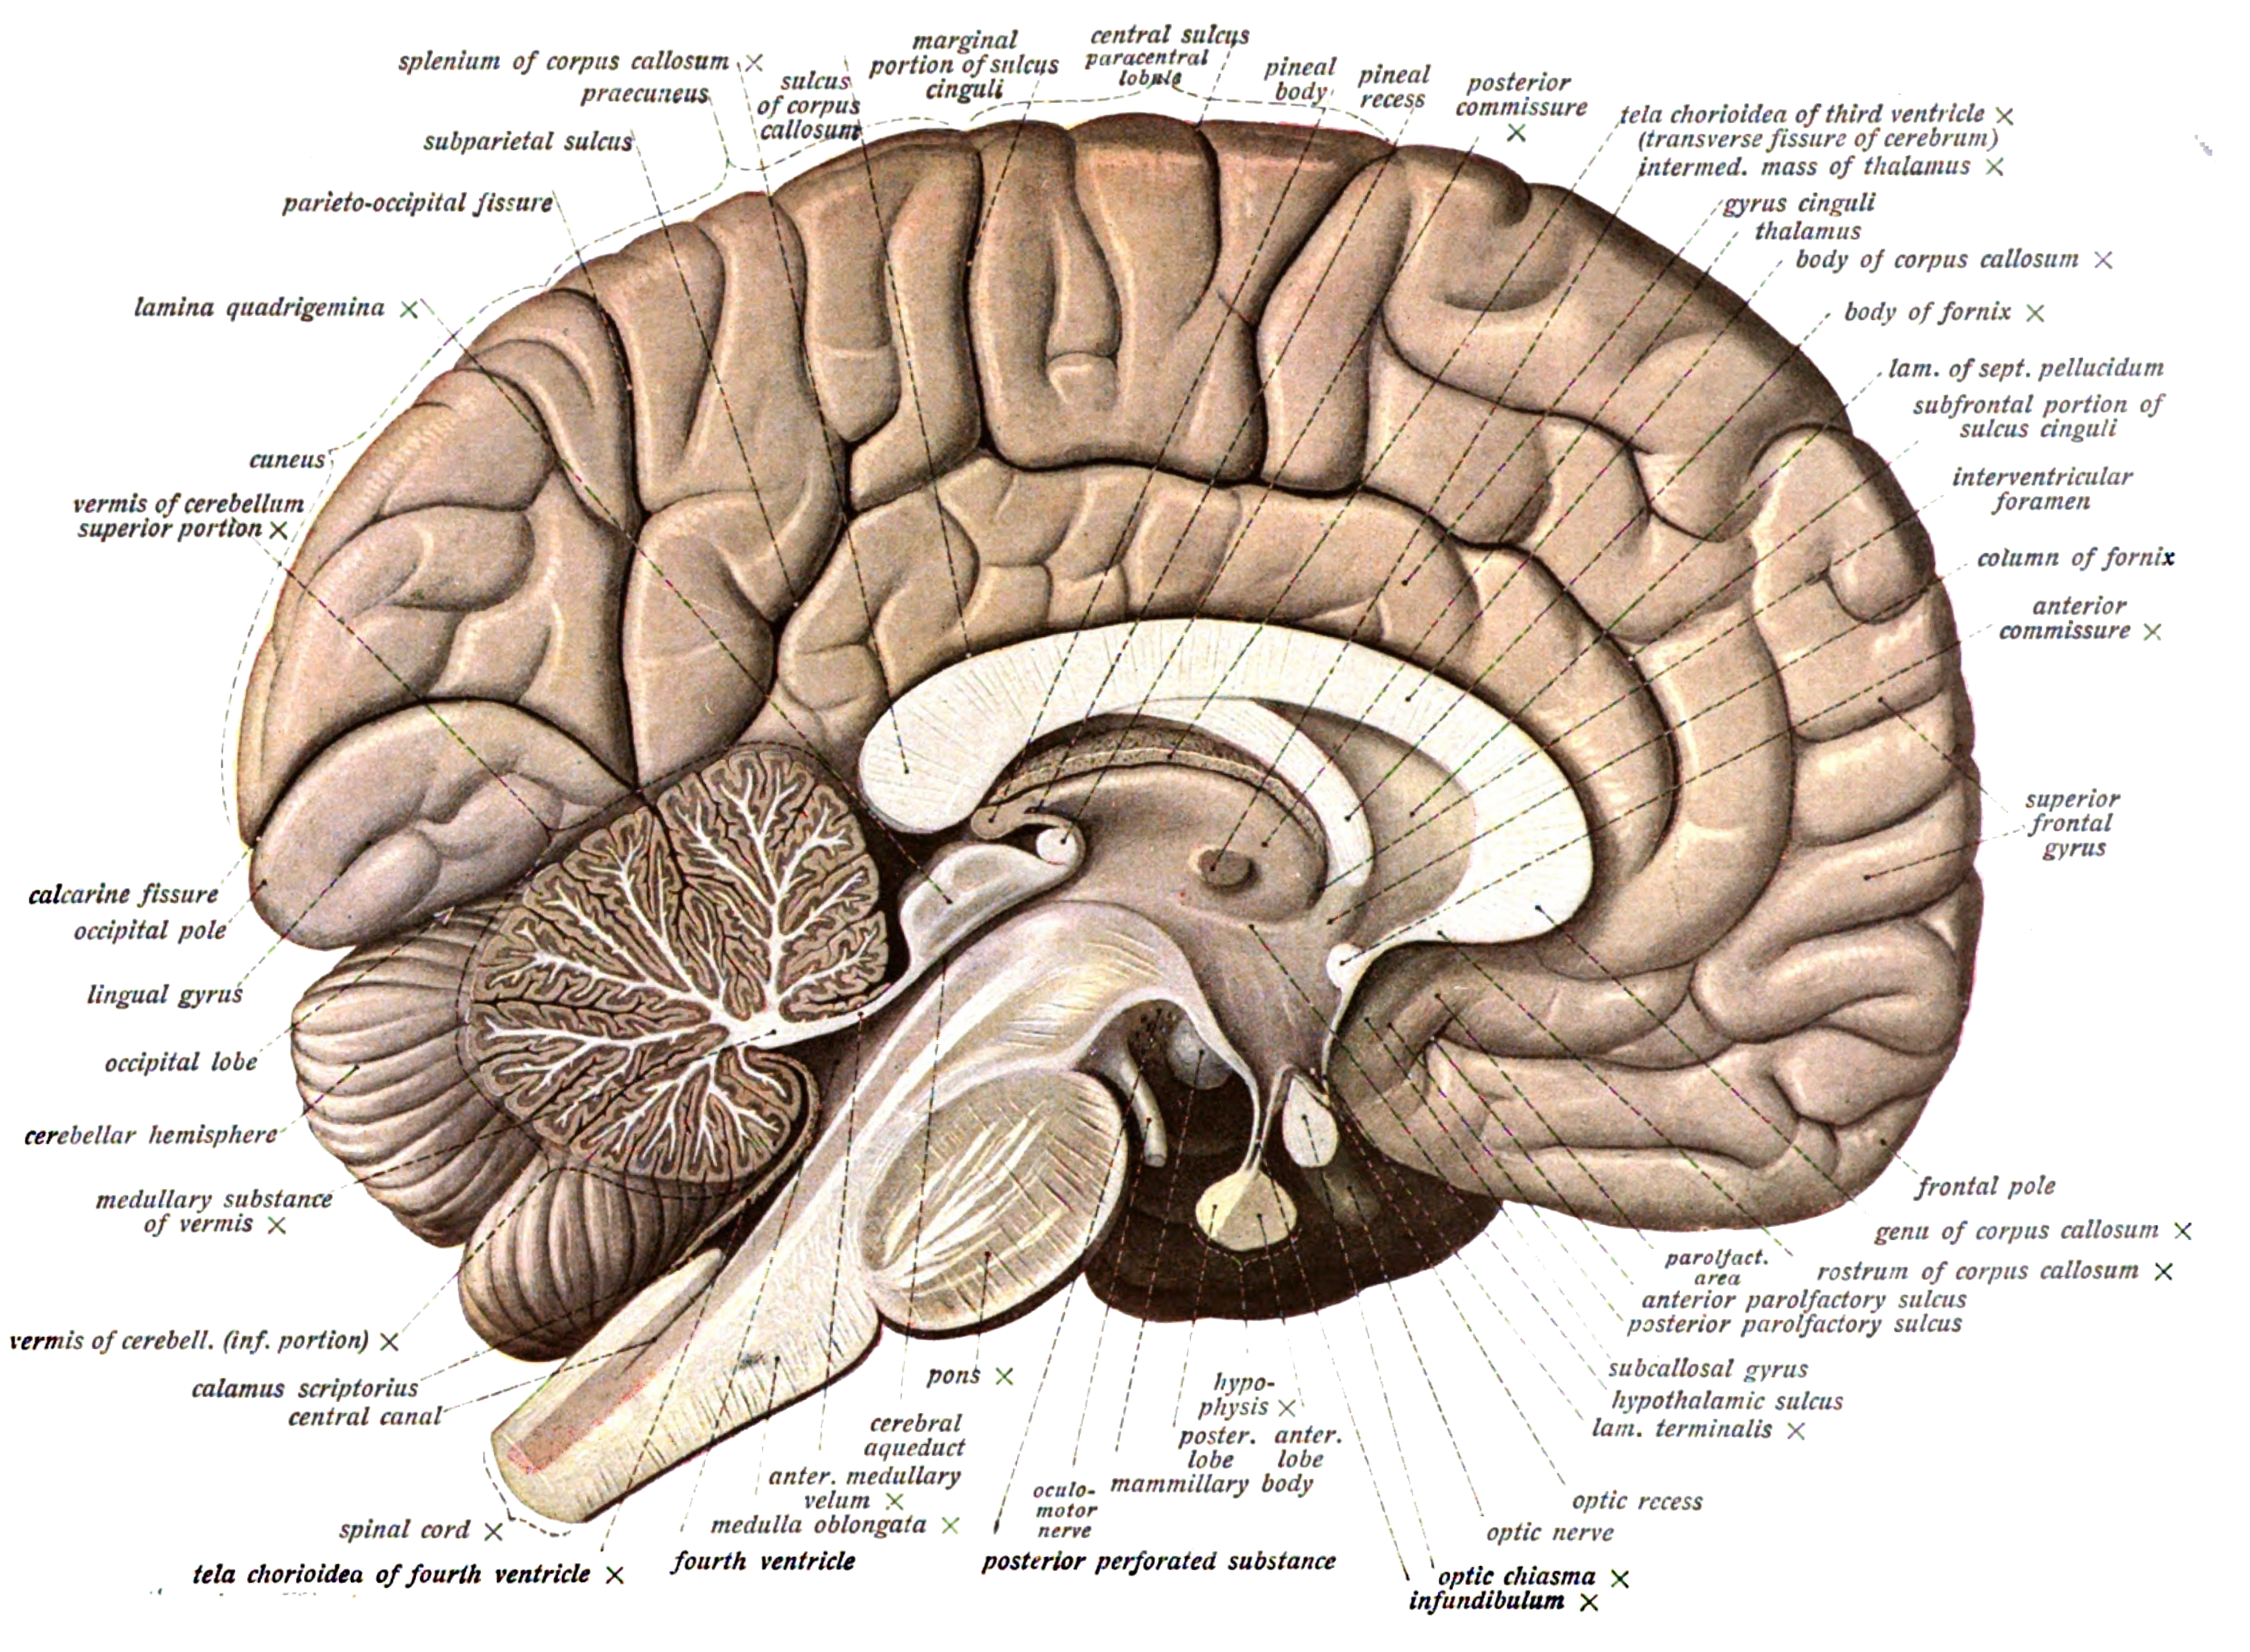
\includegraphics[width=0.9\textwidth]{Brain_Side} \\
    \normalsize
    Image from \cite{figsidebrain}.
\end{frame}


\begin{frame}[c]{The Human Brain - Different Areas}
    \includegraphics[width=0.9\textwidth]{areas_brain} \\
    \normalsize
    Roberto Biasini © 123RF.com
\end{frame}


\begin{frame}[c]{Cortical Column}
    \only<2->{
        \begin{itemize}[<+(1)->]
            \item Everywhere in the Brain
            \item 200-400 Neurons
            \item smallest symbol unit
        \end{itemize}
    }
    \only<1>{
        \includegraphics[height=0.95\textheight]{cortical_column}
        \normalsize
        Image from \cite{figcorticalcolumn}.}
\end{frame}




\begin{frame}[c]{Neuron - Number of Connections}
    \pause
    \vfill % some empty space here
    \begin{tabular}{ll}
        Min. n. of connections \phantom{AAA} & 1'000 \\
        Avg. n. of connections & 7'000 \\
        Max. n. of connections & 10'000 \\ \\ \pause
        % Min. Firing rate & 1 Hz \\
        Firing Rate & 20-250 Hz (453 Hz \cite{wang2016firing}) \\
    \end{tabular}
    \newline
    \vfill
    \small
    Connection data from \cite{herculano2009human} and firing rate from \cite{impact2015firing}.
\end{frame}


\begin{frame}[c]{Neuron - Spike Frequencies}
                                        % trim = left bottom right top
    \includegraphics[width=\textwidth, trim=0 460 750 550,clip]{spike_frequency} \\
    \normalsize
    Image adapted from \cite{yi2019average}.
\end{frame}


\begin{frame}[c]{Neuron - Overview}
    % put here: picture of neuron, focus: axons vs dendrites
    \includegraphics[width=\textwidth]{neuron} \\
    Image from \cite{figneuron}.
    % Image by <a href="https://pixabay.com/users/OpenClipart-Vectors-30363/?utm_source=link-attribution&amp;utm_medium=referral&amp;utm_campaign=image&amp;utm_content=2022398">OpenClipart-Vectors</a> from <a href="https://pixabay.com/?utm_source=link-attribution&amp;utm_medium=referral&amp;utm_campaign=image&amp;utm_content=2022398">Pixabay</a>
\end{frame}



